\documentclass[12pt]{article}

\usepackage{graphicx,color,enumerate,multicol}
\usepackage[top=1in, bottom=1in, left=1.25in, right=1.25in]{geometry}

%% Use Minion fonts if available.  Otherwise Times.
\IfFileExists{MinionPro.sty}{\usepackage[lf]{MinionPro}}{}
\usepackage{amsmath,amsthm,amsbsy}
\IfFileExists{MinionPro.sty}{}{\usepackage{times,txfonts}}

%% Setup aproblem environment, 
%% aproblem items
%% subproblems environment
%% subproblem items
\makeatletter
\newcounter{probcount}
\newcounter{subprobcount}
\newlength\probsep
\newlength\pshrinking
\newif\iffirstprob
\newenvironment{aproblems}%
  {\ifhmode\unskip\par\fi\setcounter{probcount}{0}\probsep\parskip
  \sbox\@tempboxa{\textbf{9.}}\pshrinking\wd\@tempboxa\advance\pshrinking\labelsep
  \let\hproblem\aproblem
  \advance\linewidth -\pshrinking
  \advance\@totalleftmargin\pshrinking
  \advance\leftskip\pshrinking}%
  {\ifhmode\unskip \par\fi\advance\leftskip-\pshrinking}%

\newcommand{\aproblem}{%
  \setcounter{subprobcount}{0}%
  \stepcounter{probcount}%
  \def\@currentlabel{\arabic{probcount}}%
  \ifhmode
    \unskip \par
  \fi
%  \addpenalty{-4000}%
  \iffirstprob\else\addvspace\probsep\fi
  \firstprobfalse
  \hskip -\labelwidth\hskip -\labelsep 
  \hbox to\labelwidth{\hss\textbf{\arabic{probcount}.}}\hskip\labelsep
}%

\newcommand{\subprob}{\item\def\@currentlabel{\arabic{probcount}\alph{\thelistlabel}}}
\newcommand{\skipproblem}{\stepcounter{probcount}}


%% The following commands put defined left and right headers on the top, and a page number
%% on the bottom of all pages beyond page 1
\usepackage{fancyhdr}
\pagestyle{fancy}
\fancyfoot[C]{\ifnum \value{page} > 1\relax\thepage\fi}
\fancyhead[L]{\ifx\@doclabel\@empty\else\@doclabel\fi}
\fancyhead[R]{\ifx\@docdate\@empty\else\@docdate\fi}
\headheight 15pt
\def\doclabel#1{\gdef\@doclabel{#1}}
\def\docdate#1{\gdef\@docdate{#1}}
\makeatother

%% General formatting parameters
\parindent 0pt
\parskip 6pt plus 1pt

\doclabel{Math F251: Section 2.1 Worksheet}
\docdate{22 January 2020}

\begin{document}
\renewcommand{\d}{\displaystyle}

\begin{aproblems}
\aproblem Here is a table of temperature data from NASA for years since 1990.  The first column is the year, namely the time $t$.  The second column is the difference of the globally-averaged temperature for that year minus the average of the 1951--1980 period, in Celsius.  This is the so-called \emph{temperature anomaly}, but we just regard it as a function of time.  That is, the second column contains the values of $f(t)$.

\bigskip
\hspace{-15mm}\begin{minipage}[b]{0.4\textwidth}
\footnotesize
\begin{verbatim}
        1990        0.44
        1991        0.41
        1992        0.22
        1993        0.24
        1994        0.31
        1995        0.44
        1996        0.33
        1997        0.47
        1998        0.62
        1999        0.40
        2000        0.40
        2001        0.54
        2002        0.62
        2003        0.61
        2004        0.53
        2005        0.67
        2006        0.62
        2007        0.64
        2008        0.52
        2009        0.63
        2010        0.70
        2011        0.57
        2012        0.61
        2013        0.64
        2014        0.73
        2015        0.86
        2016        0.99
        2017        0.90
        2018        0.82
\end{verbatim}
\end{minipage}
\begin{minipage}[b]{0.6\textwidth}
\qquad 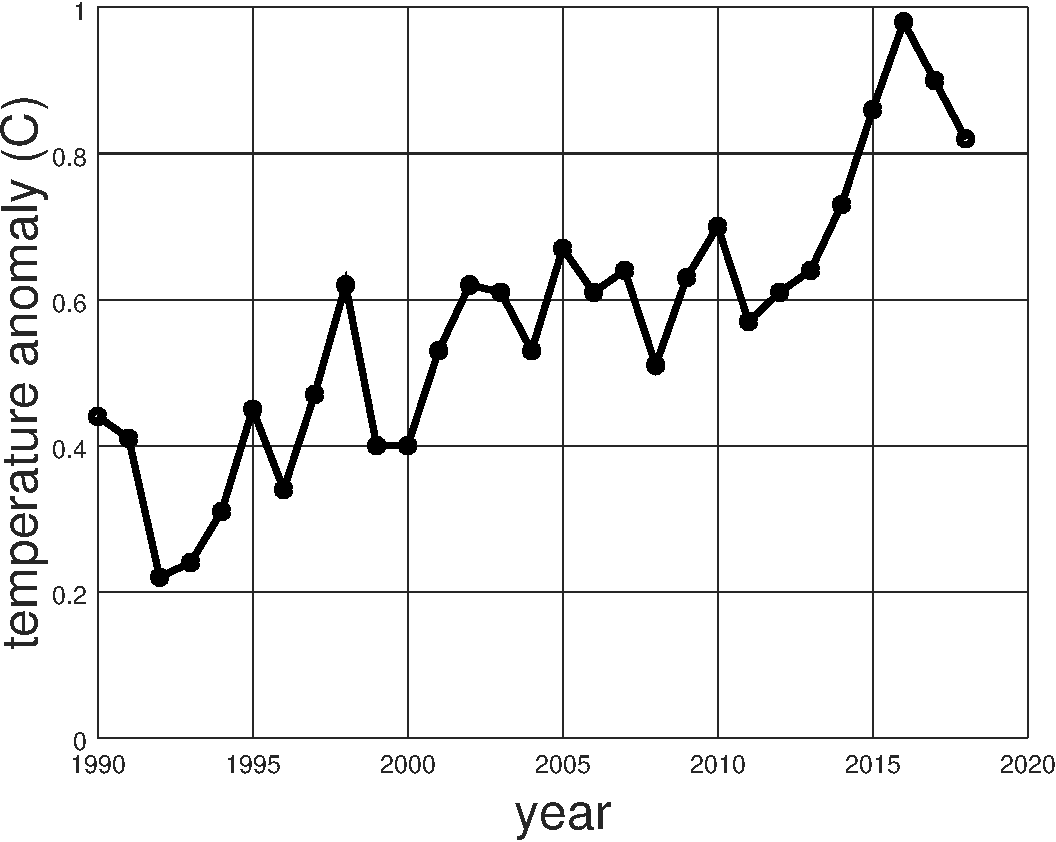
\includegraphics[width=1.05\textwidth]{tempdata/recenttemps}
\end{minipage}

\normalsize
Compute from the data:

\vspace{-5mm}
\begin{enumerate}
\item the average rate of change of temperature, i.e.~slope of the secant line for the graph of $f(t)$, in the period 1990--2018

\bigskip
\item the highest average rate of change you can compute for a ten-year period

\bigskip
\item the lowest rate of change you can compute for a ten-year period

\bigskip
\item your estimate of the rate of change in the year 2010 \hfill $\leftarrow$ \emph{answers will vary}
\end{enumerate}

\vfill
\small
\emph{This example shows that slopes can always be \emph{computed}, but noisy data does not really have a slope over a small period.  See the next page for better-behaved functions.}

\emph{Math 251 Calculus I will be \emph{entirely} about well-behaved functions; it is not real life.}
\vfill

\clearpage \newpage
\normalsize
\aproblem  (\emph{Exercise 3 in \S 2.1, simplified}.)  The point $P(2,-1)$ lies on the curve $\d y=\frac{1}{1-x}$.
\renewcommand{\labelenumi}{\alph{enumi})}
\begin{enumerate}
\item Pick a value $x$ which gives another point $Q$ on the curve.  Sketch the curve, the points $P$ and $Q$, and the secant line $PQ$.
\item Use your calculator to find the slope of the secant line $PQ$ correct to six decimal places, for the following values of $x$:
    $$\begin{matrix}
    \text{(i) 1.5} & \text{(ii) 1.99} & \text{(iii) 1.999} \\
    \\
    \text{(iv) 2.5} & \text{(v) 2.01} & \text{(vi) 2.001}
    \end{matrix}$$
\item Using the results of part a), guess the value of the slope of the tangent line to the curve at $P(2,-1)$.
\item Use the result from c) to find an equation for the tangent line at $P(2,-1)$.
\end{enumerate}
\vfill

\aproblem  (\emph{Like Exercise 2 in \S 2.1.  Compare the nice result here to the messy numbers in problem 1}.)  A cardiac monitor continuously measures the heart rate of a patient after surgery.  It compiles the number of heartbeats after $t$ minutes.  After a while it has the data below:

\begin{center}
\begin{tabular}{l|c|c|c|c|c}
$t$ (min) & 36 & 38 & 40 & 42 & 44 \\ \hline
heartbeats & 2530 &2661 & 2806 & 2948 & 3080
\end{tabular}
\end{center}

The slope of the tangent line to the graph of this data should represent the heart rate in beats per minute.  In fact the monitor estimates the heart rate using secant line slopes.

Use the data to estimate the patient's heart rate at $40$ minutes using the secant line between the points
\renewcommand{\labelenumi}{\alph{enumi})}
\begin{enumerate}
\item $t=36$ and $t=44$
\item $t=38$ and $t=42$
\item $t=38$ and $t=40$
\item $t=40$ and $t=42$
\end{enumerate}
Conclude with an estimate of the patient's heartbeat at 40 minutes.  Then add a ``$\pm x$'' statement of the uncertainty in your estimate, based on the various secant slopes above.
\vfill


\end{aproblems}

\end{document}